\chapter{व्यवहार-पारिस्थितिकी}\label{ch:b3:behavioural-ecology}

कोई मीरकैट किसी दीमक-टीले पर खड़ा रहता है जबकि उसका बाकी समूह भोजन के
लिए खोदता है, और जब कोई बाज़ दिखे तब वह भौंकता है और बाकी अपने बिलों की
ओर भागते हैं। उस प्रहरी ने घंटा भर बिना खाए बिताया है और अपने को उस
रेगिस्तान का सबसे आसानी से दिख जाने वाला प्राणी बना लिया है। क्यों? कोई
मोर ऐसी पूँछ घसीटता है जो उसके ऊर्जा-बजट का पाँचवाँ भाग लेती है और
बाघों से उसका भागना धीमा कर देती है। किसी खेत से लौटी कोई मधुमक्खी किसी
ऊर्ध्वाधर छत्ते पर नाचती है, और उसके नृत्य का ऊर्ध्वाधर से कोण उस भोजन
का सूरज से कोण है। पत्तों के किसी क्षेत्रक में इल्लियाँ खोजती कोई महा
टिटहरी उसे तब छोड़ देती है जब वहाँ अब भी इल्लियाँ मिलनी बाक़ी हैं। इनमें
से किसी प्राणी ने यह अध्याय पढ़ा नहीं, फिर भी हर एक ऐसे बरतता है मानो
उसने कोई इष्टतमन, कोई क्रीड़ा, या बंधुत्व के लेखे की कोई समस्या हल कर ली
हो। व्यवहार-पारिस्थितिकी व्यवहार का अध्ययन विकसित हुए हलों के किसी
समुच्चय के रूप में है: कोई व्यवहार किसलिए है, उन जीनों के हिसाब से
जिन्हें वह आगे बढ़ाता है, और उसकी लागतें तथा लाभ क्या होने चाहिए कि
प्राकृतिक वरण ने उसे बनाया हो। उसके औज़ार वही हैं जो कोई अर्थशास्त्री
काम में लेता है --- इष्टतमन, \omterm{prop:b3:behavioural-ecology:hawk-dove}{क्रीड़ा सिद्धांत}, संबंधिता का लेखा --- और
उसकी कसौटी क्षेत्र है।

\section{चार प्रश्न और सहजवृत्ति का तंत्र}

\begin{definition}[टिनबर्गन के प्रश्न]\label{def:b3:behavioural-ecology:tinbergen}
\index{टिनबर्गन के चार प्रश्न}\index{नियत क्रिया-प्ररूप}\index{संकेत उद्दीपक}\index{अंकन}\index{क्रांतिक काल}
टिनबर्गन (1963) ने कहा कि किसी भी व्यवहार का पूरा हिसाब चार प्रश्नों का
उत्तर देना चाहिए: उसका \emph{तंत्र} (कौन-से उद्दीपक तथा तंत्रिकीय यंत्र
उसे पैदा करते हैं), उसका \emph{परिवर्धन} (वह किसी व्यष्टि में जीनों तथा
अनुभव से कैसे उठता है), उसका \emph{प्रकार्य} (वह उत्तरजीविता तथा जनन
में क्या योग देता है) और उसका \emph{विकासीय इतिहास} (वह पुरखा व्यवहार
से कैसे उठा)। जिन आचार-विज्ञानियों ने उन्हें गढ़ा उन्होंने पहले दो जमा
दिए थे। अनेक व्यवहार \emph{नियत क्रिया-प्ररूप} हैं: किसी सरल
\emph{संकेत उद्दीपक} से छोड़े गए और एक बार शुरू होने पर पूरे चलते रूढ़
क्रम --- कोई धूसर हंस अपनी चोंच से किसी खिसके अंडे को घोंसले में वापस
लुढ़का लाता है, और उस गति को तब भी पूरा करता है जब वह अंडा बीच में हटा
दिया जाए; किसी हेरिंग गल का चूज़ा किसी भी चोंच-सरीखी वस्तु पर लाल धब्बे
को ठोंगता है, और तीन लाल पट्टियों वाली किसी छड़ी पर किसी असली गल के सिर
से अधिक ठोंगता है; और कोई नर स्टिकलबैक अपने नीचे की ओर लाल हर चीज़ पर
हमला करता है, खिड़की से दिखती किसी गुज़रती डाक-गाड़ी समेत। दूसरे किसी
खिड़की के भीतर सीखे जाते हैं: \emph{अंकन}, जिससे कोई हंस-शावक अपने पहले
दिन उसी के पीछे चलता है और उसके बाद उसी को अपना माता-पिता मानता है जो भी
चले --- कोई हंस, लोरेंज, कोई गत्ते का डिब्बा --- और जो तेज़, अनुत्क्रमणीय
तथा किसी \emph{क्रांतिक काल} तक सीमित है; और पक्षियों में गीत सीखना,
यानी वर्ष~2 के खंड का उदाहरण, उसी आकार का है। जन्मजात और सीखे हुए का
द्वंद्व झूठा है: किसी व्यवहार के पास कोई आनुवंशिक कार्यक्रम होता है जो
यह निर्दिष्ट करता है कि क्या सीखा जाना है, कब, और किससे, और विकसित वही
कार्यक्रम होता है।
\end{definition}

\begin{proof}[प्रमाण-सामग्री]
टिनबर्गन के क्षेत्र-प्रयोगों ने वह विधि गढ़ी। खोदने वाले बर्रे
(\emph{Philanthus}) रेत में छिपे किसी घोंसले तक लौटते हैं; उसने
चीड़-शंकुओं का वह वलय, जो उसने किसी एक प्रवेश के चारों ओर रखा था, उस
बर्रे के दूर रहते समय खिसका दिया, और उसने खिसके हुए वलय के केंद्र में
खोजा --- उसने वे भू-चिह्न सीखे थे। काले सिर वाले गल अंडे फूटने के बाद
घोंसले से खोल हटा देते हैं; उसने अंडों के बगल रँगे खोल, प्राकृतिक खोल
और दूसरी वस्तुएँ बिछाईं, और गिना कि कौवे कौन-से ले गए: किसी खोल का
सफ़ेद भीतरी पृष्ठ परभक्षी खींचता था, और जो हटाना सफ़ाई जैसा लगा था वह
छद्मावरण था। गल-चूज़े के प्रयोगों ने किसी \omterm{def:b3:behavioural-ecology:tinbergen}{संकेत उद्दीपक} को गत्ते के ऐसे
सिर देकर मात्राबद्ध किया जो एक बार में एक लक्षण बदलते थे। लोरेंज के
अंकित हंस उसके पीछे जीवन भर चले; और जो बतखें पहले दिन किसी चलते डिब्बे
पर अंकित हुईं वे उसके बाद किसी बतख के पीछे चलाई ही न जा सकीं।
\end{proof}

\begin{omfigure}
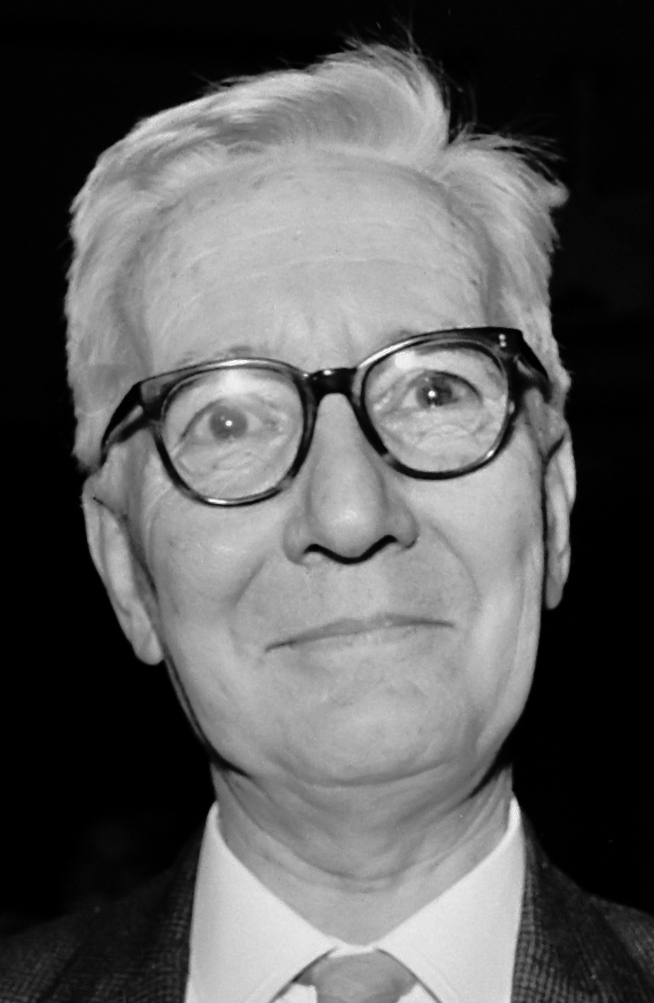
\includegraphics[width=0.36\linewidth]{images/book5/tinbergen.jpg}\hspace{0.04\linewidth}
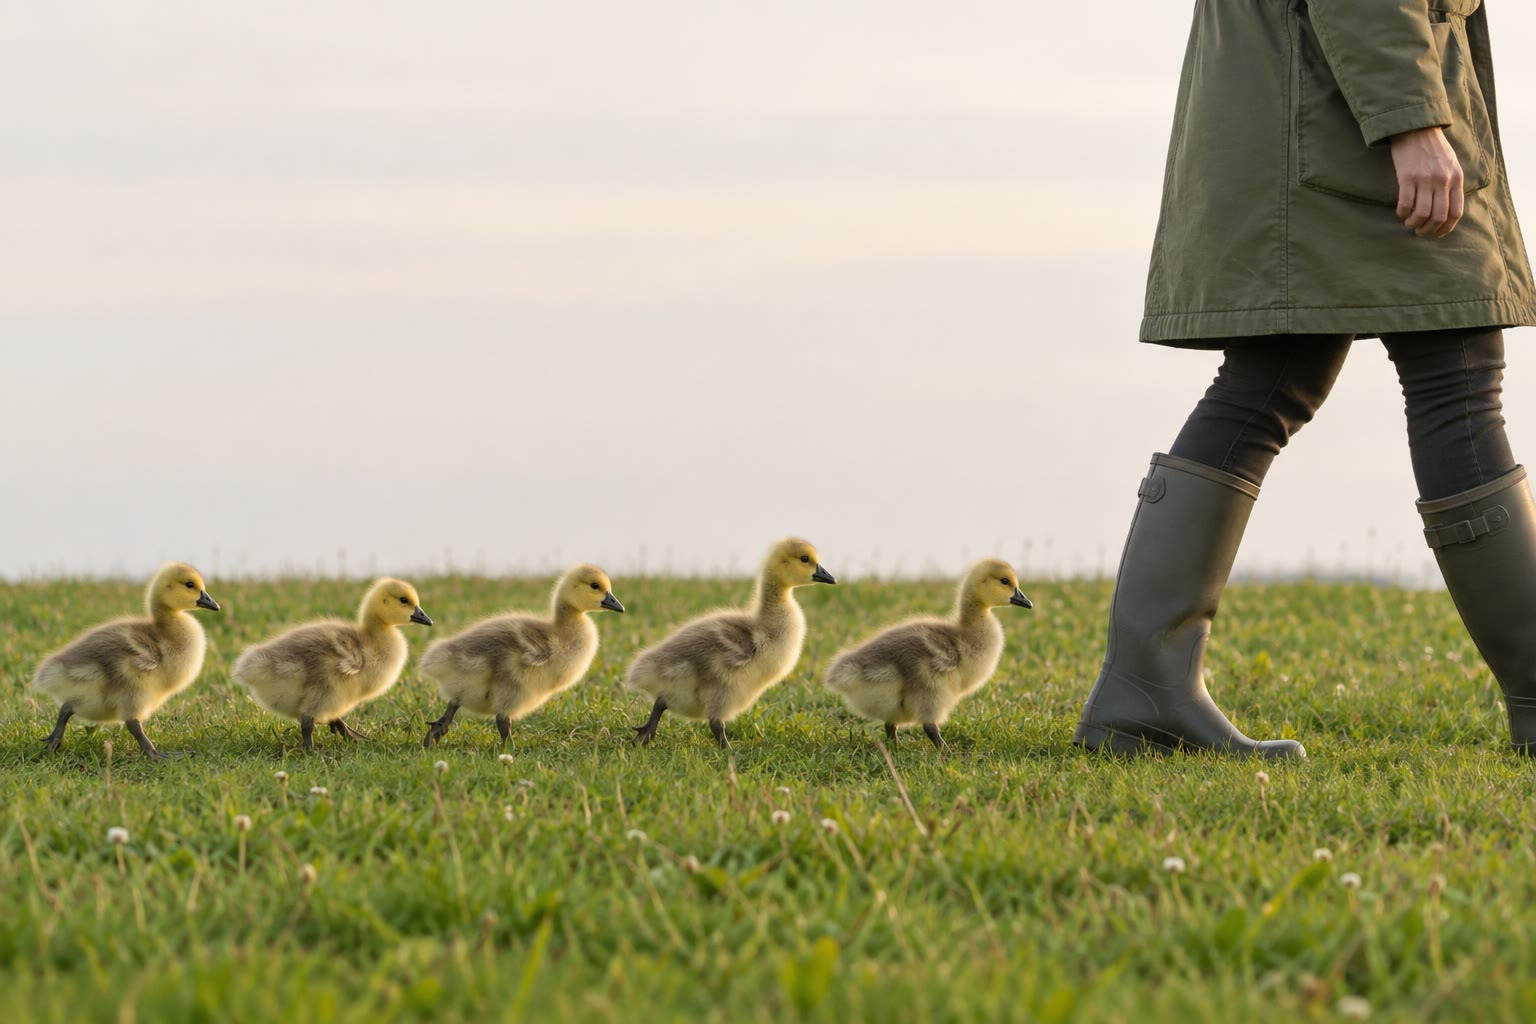
\includegraphics[width=0.52\linewidth]{images/book5/ai/b5-26-goose-imprinting.jpg}

{\small बाएँ: निको टिनबर्गन (1907--1988), जो व्यवहार के प्रश्नों को
क्षेत्र में ले गया और उन्हें प्रायोगिक बना दिया (छायाचित्र
रॉब मीरेमेट, ऐनेफ़ो, 1973, CC0)। दाएँ: फूटने के दिन भर बाद उस पहली बड़ी
चलती चीज़ के पीछे चलते हंस-शावक जो उन्होंने देखी, और जिन्हें उसके बाद
कभी और के लिए मनाया न जा सका।}
\end{omfigure}

\section{तय करना: इष्टतम आहार-खोज}

\begin{theorem}[सीमांत मूल्य प्रमेय]\label{thm:b3:behavioural-ecology:mvt}
\index{इष्टतम आहार-खोज}\index{सीमांत मूल्य प्रमेय}\index{क्षेत्रक-निवास काल}\index{मुद्रा}
कोई आहार-खोजी भोजन के उन क्षेत्रकों में जाता है जो यात्रा-काल $\tau$ से
अलग हैं। किसी क्षेत्रक में उसे ऊर्जा $g(t)$ मिलती है, समय $t$ के बाद,
जिसमें $g$ बढ़ता और नतोदर है (वह क्षेत्रक चुकता जाता है)। यदि वह हर
क्षेत्रक समय $t$ के बाद छोड़े, तो उसकी दीर्घकालिक लाभ-दर
$R(t) = g(t)/(\tau + t)$ है, और वह निवास-काल $t^{*}$, जो उसे अधिकतम करे,
यह मानता है
\[
g'(t^{*}) = \frac{g(t^{*})}{\tau + t^{*}} = R(t^{*}) :
\]
यानी किसी क्षेत्रक को तब छोड़िए जब उसमें तात्क्षणिक लाभ-दर गिरकर पूरे
आवास की औसत दर पर, यात्रा समेत, आ जाए (चार्नोव, 1976)। परिणाम: यात्रा
जितनी लंबी, ठहराव उतना लंबा और हर क्षेत्रक उतना ही पूरी तरह चुकाया
जाता है; किसी धनी आवास में (ऊँचा $R$) हर क्षेत्रक जल्दी और कम चुकाकर
छोड़ा जाता है; और सारे क्षेत्रक, उनकी गुणवत्ता जो भी हो, उसी सीमांत दर
पर छोड़े जाते हैं, इसलिए कोई कमज़ोर क्षेत्रक लगभग तुरंत छोड़ दिया जाता
है और कोई धनी तभी जब वह उस आवास के औसत तक काम कर लिया गया हो।
$g(t) = A(1 -
\mathrm{e}^{-t/T_{0}})$ के लिए वह शर्त $(\tau + t^{*})/T_{0} =
\mathrm{e}^{t^{*}/T_{0}} - 1$ बन जाती है, जो संख्यात्मक रूप से हल होती
है: $\tau = T_{0}$ के साथ $t^{*} \approx 1.15\,T_{0}$; और
$\tau = 4T_{0}$ के साथ $t^{*} \approx
2.0\,T_{0}$।
\end{theorem}
\begin{proof}
$R(t) = g(t)/(\tau + t)$; $R'(t) = [g'(t)(\tau + t) - g(t)]/(\tau +
t)^{2} = 0$ से $g'(t^{*}) = g(t^{*})/(\tau + t^{*})$ मिलता है।
ज्यामितीय रूप से: $g$ को $t$ के सामने आलेखित कीजिए, जिसका मूल-बिंदु
$-\tau$ पर हो; तब $R(t)$ उस रेखा की ढाल है जो $(-\tau, 0)$ से
$(t, g(t))$ तक जाती है, और वह वहीं अधिकतम है जहाँ वह रेखा उस वक्र की
स्पर्शी हो --- यही वह शर्त है। बड़ा $\tau$ उस मूल-बिंदु को बाईं ओर और
उस स्पर्श-बिंदु को दाईं ओर ले जाता है; और कोई धनी आवास उस स्पर्शी को
तीखा करके बाईं ओर ले जाता है। उस चरघातांक के लिए $g' = (A/T_{0})
\mathrm{e}^{-t/T_{0}}$ और $g/(\tau + t) = A(1 - \mathrm{e}^{-t/T_{0}})/
(\tau + t)$; बराबर करके फिर से सजाने पर वही दिया गया समीकरण मिलता है,
और $t^{*} = 1.15T_{0}$ रखने पर, $\tau = T_{0}$ के साथ: बायाँ $2.15$,
दायाँ $\mathrm{e}^{1.15} - 1 = 2.16$।
\end{proof}

\begin{omfigure}
\begin{tikzpicture}
\begin{axis}[
  width=0.68\linewidth, height=5.8cm,
  axis x line=middle, axis y line=left,
  xmin=-4.5, xmax=5, ymin=0, ymax=1.15,
  xlabel={समय ($T_{0}$ के मात्रकों में)}, ylabel={क्षेत्रक में मिली ऊर्जा},
  xlabel style={font=\small, at={(axis description cs:0.95,0.0)}, anchor=north}, ylabel style={font=\small},
  tick label style={font=\small}, xtick={-4,-1,0,1.15,2}, xticklabels={$-4T_0$,$-T_0$,0,$1.15$,$2.0$}, ytick={0.5,1}, yticklabels={$0.5A$,$A$},
  clip=false,
]
\addplot[very thick, omDef, domain=0:5, samples=80] {1-exp(-x)};
\draw[thick, omThm] (axis cs:-1,0) -- (axis cs:1.55,1.13);
\draw[thick, omMeth!70!black] (axis cs:-4,0) -- (axis cs:3.5,1.081);
\fill[omThm] (axis cs:1.15,0.6834) circle (2pt); \fill[omMeth!70!black] (axis cs:2,0.8647) circle (2pt);
\draw[dashed, gray] (axis cs:1.15,0) -- (axis cs:1.15,0.6834); \draw[dashed, gray] (axis cs:2,0) -- (axis cs:2,0.8647);
\node[font=\scriptsize, omThm, anchor=north west, align=left] at (axis cs:-4.4,1.1) {छोटी यात्रा, $\tau = T_{0}$:\\$t^{*} = 1.15\,T_{0}$ पर छोड़िए,\\क्षेत्रक \qty{68}{\%} चुका};
\node[font=\scriptsize, omMeth!70!black, anchor=north west, align=left] at (axis cs:2.4,0.62) {लंबी यात्रा, $\tau = 4T_{0}$:\\$t^{*} = 2.0\,T_{0}$ पर छोड़िए,\\\qty{86}{\%} चुका};
\node[font=\scriptsize, omDef, anchor=north west] at (axis cs:3.0,0.86) {$g(t) = A(1 - \mathrm{e}^{-t/T_{0}})$};
\node[font=\scriptsize, gray, anchor=south] at (axis cs:-2.5,0.02) {यात्रा};
\end{axis}
\end{tikzpicture}

{\small खींचा हुआ \omterm{thm:b3:behavioural-ecology:mvt}{सीमांत मूल्य प्रमेय}। क्षेत्रक के चुकते ही वह लाभ-वक्र
चपटा पड़ जाता है; और उस यात्रा के आरंभ से उस वक्र के किसी बिंदु तक की
रेखा की ढाल कुल लाभ-दर के बराबर है; और छोड़ने का सबसे अच्छा समय वहीं है
जहाँ वह रेखा स्पर्शी हो। कोई लंबी यात्रा उस मूल-बिंदु को बाईं ओर और उस
स्पर्श-बिंदु को दाईं ओर ले जाती है।}
\end{omfigure}

\begin{proof}[प्रमाण-सामग्री]
काउई (1977) ने किसी पक्षीशाला में महा टिटहरियों को बुरादा भरे प्यालों
में छिपे भोजन-कीड़े खोजने दिए, और प्यालों के बीच का यात्रा-काल ऐसे ढक्कन
लगाकर बदला जिन्हें हटाने में अधिक या कम समय लगता था; जब यात्रा धीमी
होती तब वे पक्षी हर प्याले में अधिक देर रुकते थे, और उस प्रमेय के
पूर्वानुमान के पीछे चलते थे, और उससे थोड़ा आगे भी निकल जाते थे, और उस
दिशा में जिसकी व्याख्या यात्रा की ऊर्जा-लागत गिनने से हो जाती है।
अपने चूज़ों के लिए लेदरजैकेट ढोती मैनाएँ (कासेलनिक, 1984) दूर रखे
भोजन-पात्रों से बड़े बोझ लेती थीं, और यह फिर वैसा ही था जैसा किसी
भरण-वक्र का दर-अधिकतमकारी हल माँगता है। इनमें से कोई भी जाँच यह सिद्ध
नहीं करती कि पक्षी स्पर्शियाँ गणित करते हैं; दोनों यह दिखाती हैं कि वरण
ने ऐसे अंगूठा-नियम बना दिए हैं जिनका परिणाम उस इष्टतम के पास है।
\end{proof}

\section{मुक़ाबले: क्रीड़ा सिद्धांत}

\begin{proposition}[बाज़--कबूतर और विकासीय रूप से स्थिर रणनीति]\label{prop:b3:behavioural-ecology:hawk-dove}
\index{क्रीड़ा सिद्धांत}\index{बाज़--कबूतर क्रीड़ा}\index{विकासीय रूप से स्थिर रणनीति}\index{बारंबारता-निर्भर वरण}
जब सबसे अच्छा व्यवहार इस पर निर्भर हो कि दूसरे क्या करते हैं, तब कोई
इष्टतम नहीं होता, केवल कोई \emph{क्रीड़ा}। दो प्राणी $V$ मूल्य के किसी
संसाधन के लिए भिड़ते हैं; कोई \emph{बाज़} तब तक लड़ता है जब तक वह घायल
(लागत $C$) या विजयी न हो, और कोई \emph{कबूतर} प्रदर्शन करता है और हमला
होने पर पीछे हट जाता है। औसत प्रतिफल हैं
\[
\begin{array}{c|cc}
 & \text{बनाम बाज़} & \text{बनाम कबूतर}\\ \hline
\text{बाज़} & (V - C)/2 & V\\
\text{कबूतर} & 0 & V/2
\end{array}
\]
कोई \emph{\omterm{prop:b3:behavioural-ecology:hawk-dove}{विकासीय रूप से स्थिर रणनीति}} (मेनार्ड स्मिथ और प्राइस, 1973)
वह है जिस पर, एक बार आम हो जाने पर, किसी भी बिरले विकल्प का हमला नहीं
हो सकता। यदि $V > C$ हो, तो बाज़ ही ESS है: लड़ना लड़ाकों के सामने भी
फ़ायदेमंद है। यदि $V
< C$ हो, तो कोई भी शुद्ध रणनीति स्थिर नहीं --- कबूतरों की किसी समष्टि
पर बाज़ हमला कर देते हैं, जो हर मुक़ाबला जीतते हैं, और बाज़ों की किसी
समष्टि पर कबूतर, जो चोटों से बच जाते हैं --- और ESS यह है कि बाज़
प्रायिकता
\[
p^{*} = \frac{V}{C},
\]
से खेला जाए, या, तुल्य रूप से, कोई ऐसी समष्टि जिसमें वही अंश बाज़ हों।
उस ESS पर दोनों रणनीतियाँ बराबर अच्छा करती हैं, और हर एक औसतन $V(1 -
V/C)/2$ पाती है, जो उस $V/2$ से कम है जो कबूतरों की कोई समष्टि
बाँटती: वह मुक़ाबला सबको महँगा पड़ता है, और कोई अकेला उससे बेहतर नहीं कर
सकता। यहाँ वरण \emph{बारंबारता-निर्भर} है: किसी रणनीति की सुयोग्यता उसके
आम होते ही गिरती है, और इसीलिए प्राणियों के मुक़ाबले अधिकांशतः प्रदर्शन
हैं और कभी-कभी युद्ध, और इसीलिए वह मिश्रण टिका रहता है।
\end{proposition}
\begin{proof}
मान लीजिए अंश $p$ बाज़ खेलता है। किसी बाज़ का प्रत्याशित प्रतिफल
$W_{H} = p(V
- C)/2 + (1 - p)V$ है; किसी कबूतर का $W_{D} = (1 - p)V/2$।
$W_{H} - W_{D} =
p(V - C)/2 + (1 - p)V/2 = [V - pC]/2$, जो $p < V/C$ के लिए धनात्मक है
और उससे ऊपर ऋणात्मक: बाज़ बिरले होने पर फैलते हैं और आम होने पर छँट
जाते हैं, और वह बारंबारता वहाँ जम जाती है जहाँ $W_{H} = W_{D}$ हो,
यानी $p^{*} = V/C$ पर। कि वह स्थिर है, यह उस चिह्न-बदलाव से निकलता है:
$p$ का $p^{*}$ से ऊपर कोई विक्षोभ कबूतरों का पक्ष लेता है और सुधर जाता
है, और उससे नीचे बाज़ों का। यदि $V
\ge C$ हो तो वह अंतर हर $p \le 1$ के लिए धनात्मक है और बाज़ स्थिर हो
जाता है। $p^{*}$ पर साझा प्रतिफल: $W_{D} = (1 - V/C)V/2$।
\end{proof}

\begin{omfigure}
\begin{tikzpicture}
\begin{axis}[
  width=0.6\linewidth, height=5.4cm,
  axis x line=bottom, axis y line=left,
  xmin=0, xmax=1, ymin=-1, ymax=4.2,
  xlabel={बाज़ों का अंश $p$}, ylabel={प्रत्याशित प्रतिफल},
  xlabel style={font=\small, at={(axis description cs:0.5,-0.12)}, anchor=north}, ylabel style={font=\small},
  tick label style={font=\small}, xtick={0,0.5,1}, xticklabels={0,$p^{*} = V/C$,1}, ytick={0,1,2,4},
  clip=false,
]
\addplot[very thick, omThm, domain=0:1, samples=2] {x*(4-8)/2 + (1-x)*4};
\addplot[very thick, omDef, domain=0:1, samples=2] {(1-x)*4/2};
\draw[dashed, gray] (axis cs:0.5,-1) -- (axis cs:0.5,1);
\fill[black] (axis cs:0.5,1) circle (2pt);
\node[font=\scriptsize, omThm, anchor=north west] at (axis cs:0.5,3.9) {बाज़: $p(V - C)/2 + (1 - p)V$};
\node[font=\scriptsize, omDef, anchor=south west] at (axis cs:0.62,0.9) {कबूतर: $(1 - p)V/2$};
\node[font=\scriptsize, anchor=west, align=left] at (axis cs:0.55,2.6) {$V = 4$, $C = 8$:\\$p^{*} = 0.5$ पर ESS,\\प्रतिफल $V(1 - V/C)/2 = 1$};
\draw[->, thick, omThm] (axis cs:0.1,-0.5) -- (axis cs:0.4,-0.5); \draw[->, thick, omDef] (axis cs:0.9,-0.5) -- (axis cs:0.6,-0.5);
\node[font=\tiny, anchor=north] at (axis cs:0.25,-0.55) {बाज़ फैलते}; \node[font=\tiny, anchor=north] at (axis cs:0.75,-0.55) {कबूतर फैलते};
\end{axis}
\end{tikzpicture}

{\small \omterm{prop:b3:behavioural-ecology:hawk-dove}{बाज़--कबूतर क्रीड़ा}। जहाँ वे प्रतिफल-रेखाएँ काटती हैं वहाँ दोनों
रणनीतियाँ बराबर अच्छा करती हैं और कोई फैल नहीं सकती; और दोनों ओर वरण
उस बारंबारता को वापस धकेल देता है। वह मिश्रण स्थिर है और सबको महँगा
पड़ता है, और प्राणियों के मुक़ाबले ऐसे ही दिखते हैं।}
\end{omfigure}

\begin{example}[क्षेत्र में क्रीड़ाएँ]\label{ex:b3:behavioural-ecology:games}
नर चित्तीदार वन-तितलियाँ वन-तल के धूप-धब्बों के लिए भिड़ती हैं: कोई
छोटी सर्पिल उड़ान लगभग हमेशा निवासी जीतता है, और जब दो नरों को इस
भ्रम में डाला जाए कि हर एक अपने को निवासी माने तब वह लड़ाई दस गुना लंबी
चलती है --- यानी कोई रूढ़ि (``निवासी जीतता है'') जो मुक़ाबले सस्ते में
निपटा देती है, और जो स्वयं कोई ESS है जब लड़ना महँगा हो और वह संसाधन
अधिक मूल्य का न हो। नर गोबर-मक्खियाँ मादाओं के लिए गोबर-थापों पर
प्रतीक्षा करती हैं और तब छोड़ देती हैं जब आगमनों की दर गिरकर उतनी रह
जाए जितनी कोई ताज़ा थाप देती --- यानी फिर वही \omterm{thm:b3:behavioural-ecology:mvt}{सीमांत मूल्य प्रमेय}, किसी
ऐसी क्रीड़ा में जिसमें उस क्षेत्रक का मूल्य इस पर निर्भर है कि उस पर
कितने प्रतिद्वंद्वी बैठे हैं। अंजीर-बर्रे, वे धब्बेदार छिपकलियाँ जिनके
तीन नर-प्ररूप एक-दूसरे को चक्रीय रूप से पत्थर--कागज़--कैंची की तरह
हराते हैं, और सामन तथा ब्लूगिल सनफ़िश के वे ``चोरिया'' नर, जो उन क्षेत्री
नरों के पास से लपककर अंडे निषेचित कर देते हैं जिनसे वे लड़ नहीं सकते,
सब ऐसे मिश्रण हैं जो उन बारंबारताओं पर थमे हैं जहाँ वे विकल्प बराबर
फ़ायदा देते हैं। क्षय-युद्ध --- दो प्राणी तब तक प्रदर्शन करते हैं जब तक
एक हार न मान ले, और ESS यह है कि किसी चरघातांकी वितरण से खींचे गए किसी
यादृच्छिक समय तक डटा जाए --- अनेक जातियों के घूरने के मुक़ाबलों का वर्णन
करता है, और सही-सही यह पूर्वानुमान करता है कि हारने वाले का डटना इस
बारे में कुछ नहीं बताता कि वह कितनी देर और चलता।
\end{example}

\section{बंधु: हैमिल्टन का नियम}

\begin{theorem}[हैमिल्टन का नियम]\label{thm:b3:behavioural-ecology:hamilton}
\index{हैमिल्टन का नियम}\index{बंधु-वरण}\index{संबंधिता}\index{समावेशी सुयोग्यता}\index{परोपकारिता}\index{अगुणित-द्विगुणिता}
कोई ऐसा युग्मविकल्पी, जो अपने वाहक से कोई ऐसा काम करवाए जो उसे $c$
संतति की लागत दे और किसी संबंधी को $b$ अतिरिक्त संतति दे, तब फैलता है जब
\[
r\,b > c ,
\]
जहाँ $r$ \emph{संबंधिता का गुणांक} है: यानी यह प्रायिकता कि ग्रहीता का
कोई जीन उसी जीन की, वंशागति से, कोई प्रति है जो उस कर्ता में है ---
माता-पिता तथा संतति या सगे भाई-बहनों के लिए $1/2$, सौतेले भाई-बहनों,
नाती-पोतों, भतीजी-भतीजों के लिए $1/4$, और पहले चचेरों के लिए $1/8$। वह
राशि जिसे वह युग्मविकल्पी अधिकतम करता है उसके वाहक की \emph{\omterm{thm:b3:behavioural-ecology:hamilton}{समावेशी
सुयोग्यता}} है: यानी उसका अपना जनन जमा संबंधियों के जनन पर उसके असर, और हर
एक $r$ से भारित। इस तरह \emph{परोपकारिता} --- यानी ऐसा व्यवहार जो कर्ता
का जनन घटाए और किसी दूसरे का बढ़ाए --- बंधुओं की ओर, संबंधिता के
अनुपात में विकसित होती है, और वह नियम यह पूर्वानुमान करता है कि वह कहाँ
मिलनी चाहिए: मादा भू-गिलहरियों की चेतावनी-पुकारों में, जो अपनी बहनों तथा
बेटियों के बीच रहती हैं, और उन नरों की नहीं, जो बिखर जाते हैं;
मीरकैटों की प्रहरी-ड्यूटी में, जिनका समूह कोई परिवार है; और उन पक्षियों
के घोंसले पर मददगारों में जो क्षेत्रों के भर जाने पर अपने माता-पिता की
भाई-बहन पालने में मदद करते हैं। \emph{अगुणित-द्विगुणित} हाइमेनॉप्टेरा
में --- जिनके नर अनिषेचित अंडों से गुणसूत्रों के एक ही समुच्चय के साथ
आते हैं और मादाएँ दो के साथ --- सगी बहनें अपने जीनों का तीन-चौथाई साझा
करती हैं ($r = 3/4$), जो उससे अधिक है जितना कोई माँ अपनी बेटियों से साझा
करती है ($1/2$), और हैमिल्टन ने इसे यह कारण बताया कि चींटियों,
मधुमक्खियों तथा बर्रों के बंध्य श्रमिक-वर्ग वहाँ ग्यारह बार उठे और
अन्यत्र लगभग कभी नहीं।
\end{theorem}
\begin{proof}
उस युग्मविकल्पी की प्रतियों पर विचार कीजिए। जब वह कर्ता वह काम करता है,
तब उसकी अपनी प्रतियाँ प्रत्याशित संचरण में $c$ खो देती हैं; और वह
ग्रहीता उस युग्मविकल्पी को समष्टि के औसत से $r$ ऊपर की प्रायिकता से
ढोता है, इसलिए उस ग्रहीता का लाभ $b$ उस युग्मविकल्पी का संचरण औसतन
$rb$ बढ़ा देता है। वह युग्मविकल्पी तब बारंबारता में बढ़ता है जब
$rb - c > 0$ हो (हैमिल्टन, 1964; और सामान्य व्युत्पत्ति, जो किसी
व्यष्टि के जीनरूप तथा उसकी सुयोग्यता के बीच के सहप्रसरण से आती है, प्राइस
समीकरण है, जो यहाँ स्वीकार कर लिया गया है)। संबंधिता: कोई माता-पिता हर
जीन किसी संतति को प्रायिकता $1/2$ से संचरित करता है; दो सगे भाई-बहनों में
से हर एक ने कोई दिया जीन उसी एक माता-पिता से प्रायिकता $1/2$ से पाया,
और वह वही प्रति है प्रायिकता $1/2$ से, और माता-पिता दो हैं:
$r = 2\times\tfrac{1}{2}
\times\tfrac{1}{2} = \tfrac{1}{2}$। अगुणित-द्विगुणित बहनें: अपने
अगुणित पिता से वे एक जैसे जीन पाती हैं (प्रायिकता $1$); और अपनी माँ से
एक जैसी प्रतियाँ प्रायिकता $1/2$ से; और दोनों माता-पिता पर औसत लेने पर,
$r = (1 + 1/2)/2 = 3/4$।
\end{proof}

\begin{omfigure}
\begin{tikzpicture}[every node/.style={font=\scriptsize}, >=stealth]
  % diploid pedigree
  \node[draw, circle, fill=omDef!30, minimum size=6mm] (m) at (0,3) {}; \node[draw, fill=omDef!30, minimum size=6mm] (f) at (1.6,3) {};
  \node[above, font=\tiny] at (0.8,3.4) {द्विगुणित माता-पिता};
  \draw[thick] (m) -- (f);
  \node[draw, circle, fill=omThm!40, minimum size=6mm] (a) at (0,1.5) {}; \node[draw, circle, fill=omDef!15, minimum size=6mm] (s) at (1.6,1.5) {};
  \draw[thick] (0.8,3) -- (0.8,2.2) -- (0,2.2) -- (a); \draw[thick] (0.8,2.2) -- (1.6,2.2) -- (s);
  \node[draw, circle, fill=omDef!15, minimum size=6mm] (c) at (1.6,0) {}; \draw[thick] (s) -- (c);
  \node[draw, circle, fill=omDef!15, minimum size=6mm] (o) at (0,0) {}; \draw[thick] (a) -- (o);
  \node[left, omThm, font=\tiny] at (-0.4,1.5) {कर्ता};
  \node[right, font=\tiny] at (1.95,1.5) {सगा भाई-बहन: $r = 1/2$};
  \node[right, font=\tiny] at (1.95,0) {भतीजी: $r = 1/4$};
  \node[left, font=\tiny] at (-0.4,0) {अपनी संतति: $1/2$};
  \node[right, font=\tiny] at (1.95,3) {माता-पिता: $r = 1/2$};
  % haplodiploid
  \begin{scope}[shift={(7.2,0)}]
    \node[draw, circle, fill=omDef!30, minimum size=6mm] (q) at (0,3) {}; \node[draw, fill=omMeth!40, minimum size=6mm] (d) at (1.6,3) {};
    \node[above left, font=\tiny] at (0.1,3.3) {रानी (द्विगुणित)}; \node[above right, font=\tiny] at (1.5,3.3) {ड्रोन (अगुणित)};
    \draw[thick] (q) -- (d);
    \node[draw, circle, fill=omThm!40, minimum size=6mm] (w) at (0,1.5) {}; \node[draw, circle, fill=omDef!15, minimum size=6mm] (w2) at (1.6,1.5) {};
    \draw[thick] (0.8,3) -- (0.8,2.2) -- (0,2.2) -- (w); \draw[thick] (0.8,2.2) -- (1.6,2.2) -- (w2);
    \node[left, omThm, font=\tiny] at (-0.4,1.5) {श्रमिक};
    \node[right, align=left, font=\tiny] at (1.95,1.5) {सगी बहन: $r = 3/4$\\(पिता के जीन एक जैसे,\\माँ के $1/2$ से साझा)};
    \node[draw, circle, fill=omDef!15, minimum size=6mm] (wd) at (0,0) {}; \draw[thick] (w) -- (wd);
    \node[right, font=\tiny] at (0.35,0) {अपनी बेटी: $1/2$ --- किसी बहन से कम};
  \end{scope}
  \node[below, align=center] at (4.6,-0.9) {हैमिल्टन का नियम: तब मदद कीजिए जब $r\,b > c$; कोई अगुणित-द्विगुणित श्रमिक बहनें पालकर\\प्रति संतति अपने अधिक जीन आगे बढ़ाती है, बजाय बेटियाँ पालने के};
\end{tikzpicture}

{\small दो तरह के परिवारों में संबंधिता। किसी द्विगुणित वंशावली में कोई
भाई-बहन आधी संतति के बराबर है; और किसी अगुणित-द्विगुणित बस्ती में कोई
बहन किसी बेटी से अधिक मूल्य की है, जो उस अंकगणित को घर पर रुककर मदद
करने की ओर झुका देता है।}
\end{omfigure}

\begin{proof}[प्रमाण-सामग्री]
शर्मन (1977) ने तीन गर्मियाँ बेल्डिंग की भू-गिलहरियाँ देखीं और दर्ज
किया कि आते परभक्षियों पर चेतावनी-पुकार कौन देता है: जिन मादाओं के पास
बंधु थे वे उन मादाओं से, जिनके पास नहीं थे, और उन नरों से, जो अपनी
जन्मभूमि से बिखर चुके थे और जिनका कोई संबंधी सुनने की दूरी में नहीं था,
कहीं अधिक बार पुकारती थीं --- उस पुकारने वाले ने उस परभक्षी का ध्यान
खींचा, और उसकी क़ीमत चुकाई, केवल तभी जब चेताने को संबंधी थे। एमलन के
सफ़ेद-मुँह पतरिंगे घोंसले पर संबंधिता के अनुपात में मदद करते हैं, और
उपलब्ध घोंसलों में से निकटतम बंधुओं के चुनते हैं। क्लटन-ब्रॉक के
दीर्घकालिक मीरकैट अध्ययन ने पाया कि प्रहरी वे अच्छी तरह खाए व्यष्टि होते
हैं जिनके पास खोने को सबसे कम है, और कि उस समूह की --- और इसलिए उस
प्रहरी के संबंधियों की --- उत्तरजीविता प्रहरी-प्रयास के साथ चढ़ती है;
पर वह लागत उससे छोटी निकली जितनी वह कहानी मानती थी, क्योंकि किसी टीले
पर बैठा प्रहरी प्रायः बिल तक पहुँचने वाला पहला होता है।
\end{proof}

\begin{omfigure}
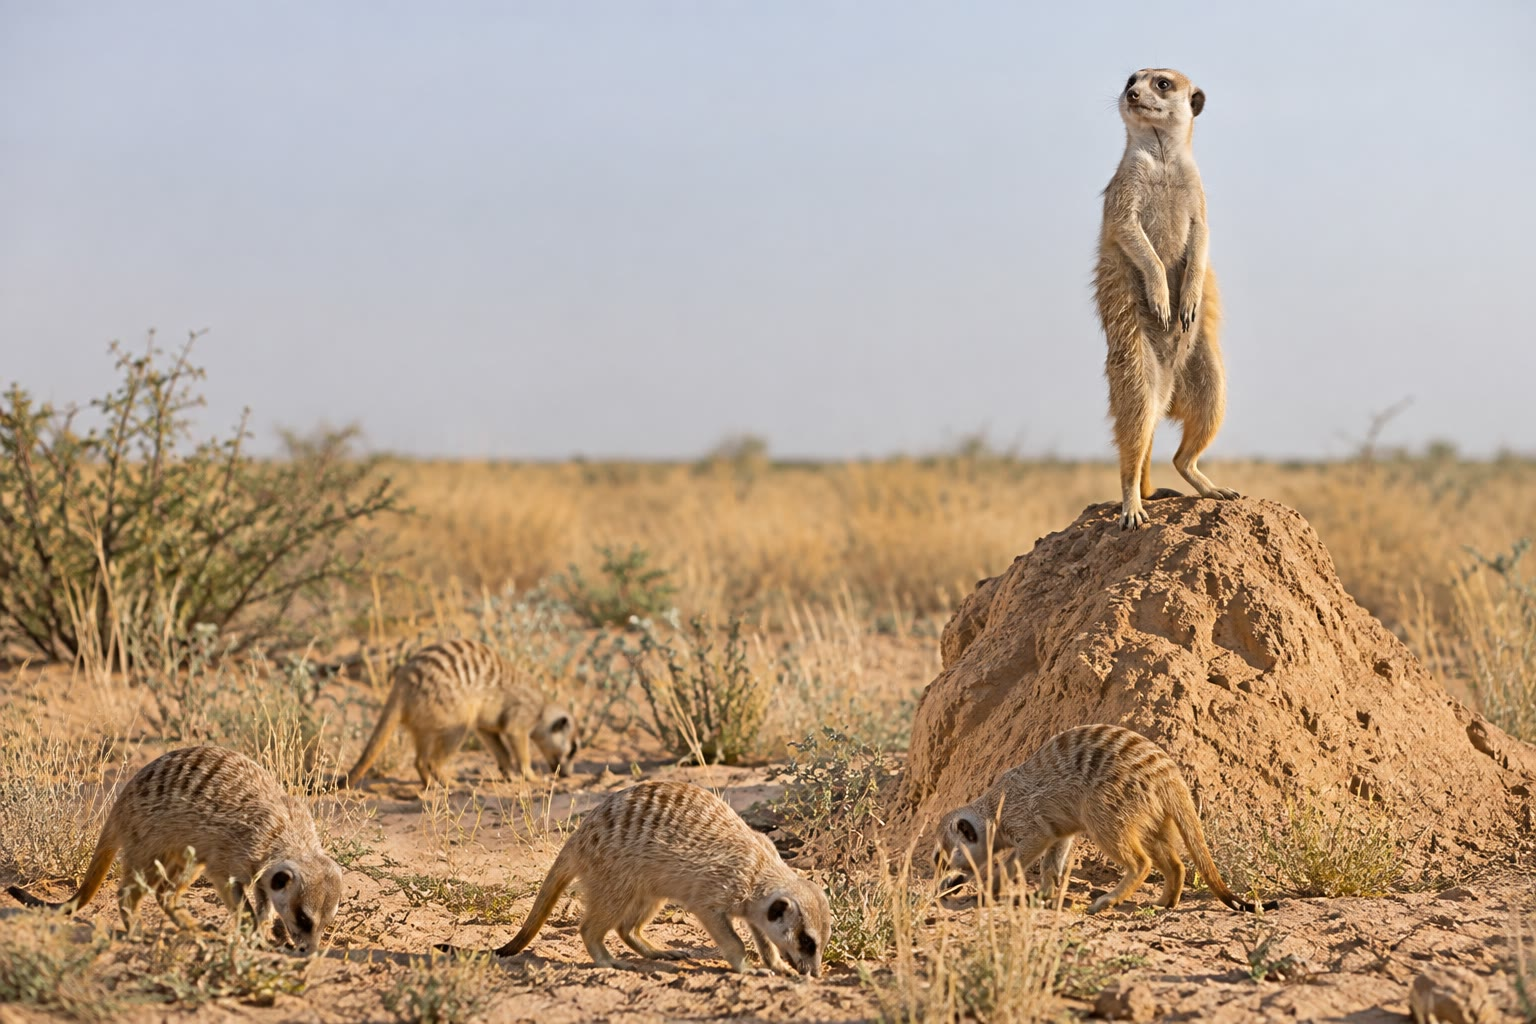
\includegraphics[width=0.46\linewidth]{images/book5/ai/b5-26-meerkat-sentinel.jpg}\hspace{0.04\linewidth}
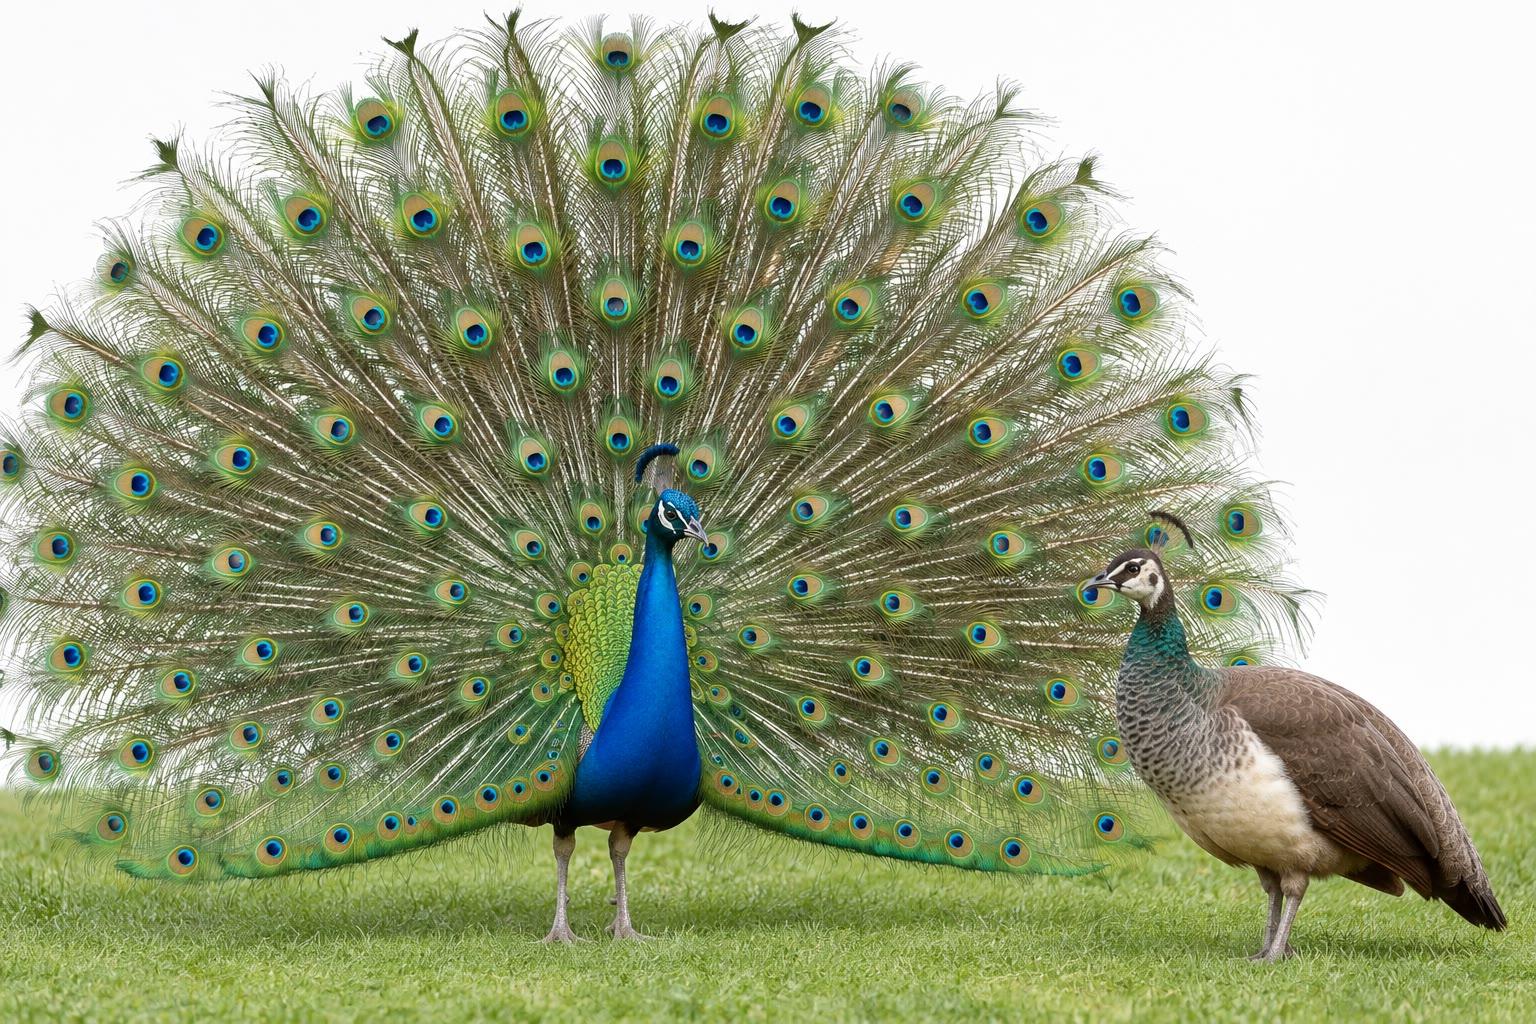
\includegraphics[width=0.46\linewidth]{images/book5/ai/b5-26-peacock-display.jpg}

{\small बाएँ: अपने संबंधियों के किसी आहार खोजते समूह के ऊपर
प्रहरी-ड्यूटी पर बैठा कोई मीरकैट। दाएँ: किसी मोरनी के सामने प्रदर्शन
करता कोई मोर --- यानी कोई ऐसी संरचना जो अपने वाहक को भोजन तथा गति में
महँगी पड़ती है और उसे उसके ध्यान के सिवा कुछ नहीं दिलाती।}
\end{omfigure}

\section{जोड़े और संदेश}

\begin{definition}[लैंगिक वरण]\label{def:b3:behavioural-ecology:sexual-selection}
\index{लैंगिक वरण}\index{बेटमैन प्रवणता}\index{भगोड़ा वरण}\index{बाधा-सिद्धांत}\index{अच्छे जीन}\index{लैंगिक संघर्ष}
डार्विन का दूसरा तंत्र: उन लक्षणों पर वरण जो उत्तरजीविता के बजाय जोड़े
जिताएँ। उसकी जड़ असमयुग्मकता है --- किसी मादा का जनन उन अंडों से सीमित है
जो वह बना और भर सकती है, और किसी नर का उन मादाओं से जिन्हें वह निषेचित
कर सकता है --- ताकि अधिकांश जातियों में किसी नर की सुयोग्यता उसके संगमों की
संख्या के साथ तीखी चढ़े और किसी मादा की मुश्किल से (यानी \emph{बेटमैन
प्रवणता}); तब नर मादाओं के लिए स्पर्धा करते हैं और मादाएँ नरों में से
चुनती हैं। स्पर्धा सींग, विषाण, दाँत, बड़ा आकार और पिछले खंड के
मुक़ाबले देती है। चुनाव आभूषण देता है, और इसके तीन हिसाब कि मादाएँ
उन्हें क्यों पसंद करती हैं। फ़िशर का \emph{भगोड़ा}: थोड़ी लंबी पूँछ की
पसंद और वह लंबी पूँछ साथ-साथ फैले, और हर एक दूसरे को लाभदायक बनाती गई,
जब तक उस पूँछ की उत्तरजीविता-लागत उसके संगम-लाभ को संतुलित न कर दे।
ज़हावी की \emph{बाधा}: कोई ऐसा आभूषण जिसे केवल कोई स्वस्थ नर उगाने का
ख़र्च उठा सके, उसकी दशा का कोई \omterm{prop:b3:behavioural-ecology:signals}{ईमानदार संकेत} है, ठीक इसीलिए कि वह महँगा
है --- और पूरी पूँछ वाले किसी मोर में, प्रत्यक्ष रूप से, कम परजीवी होते
हैं। \emph{अच्छे जीन} और \emph{सीधे लाभ}: वह मादा अपनी संतति की
वंशागति के ज़रिए या उस क्षेत्र तथा भोजन के ज़रिए पाती है जो वह नर देता
है। दोनों लिंगों के हित भिन्न हैं, और \emph{लैंगिक संघर्ष} --- संगम की
बारंबारता पर, इस पर कि शिशुओं की देखभाल कौन करे, किसी पिछले जोड़े के
शुक्राणुओं की नियति पर --- किसी एक ही जाति के भीतर चलती कोई होड़ है: नर
फल-मक्खियों का शुक्रीय द्रव उस मादा का जीवन छोटा कर देता है और उसका
अंडा देना बढ़ा देता है, और मादाएँ प्रतिरोध विकसित करती हैं।
\end{definition}

\begin{proof}[प्रमाण-सामग्री]
ऐंडरसन (1982) ने केन्या में नर लंबी-पूँछ विडोबर्डों के पूँछ-पंख काटे
और चिपकाए: जिन नरों की पूँछ उनकी प्राकृतिक लंबाई से दुगुनी की गई
उन्होंने अपने क्षेत्रों में उन नरों से चार गुना नए घोंसले खींचे जिनकी
पूँछें छोटी की गई थीं, जबकि वे नियंत्रण, जिनकी पूँछें काटकर बिना बदले
वापस चिपका दी गईं, अप्रभावित रहे --- यानी किसी भी नर की उगती पूँछ से
लंबी पूँछ के लिए मादा की पसंद, जो उस लक्षण से आगे वरित किसी पसंद का
हस्ताक्षर है। पेट्री (1994) ने पाया कि मोरनियाँ उन्हीं नरों से संगम
करती थीं जिनकी पूँछों पर सबसे अधिक आँख-धब्बे थे, और कि उन्हीं नरों के
चूज़े उन जंगलों में बेहतर बचे जहाँ वे छोड़े गए --- यानी कोई नापा गया
अच्छे-जीन लाभ। बेटमैन (1948) ने चिह्नक उत्परिवर्तन ढोती फल-मक्खियों के
संगम तथा संतति गिने और वह प्रवणता पाई जो उसका नाम ढोती है: नर की
जनन-सफलता संगमों के साथ रैखिक रूप से चढ़ी, और मादा की एक के बाद पठार पर
आ गई।
\end{proof}

\begin{proposition}[ईमानदार संकेत]\label{prop:b3:behavioural-ecology:signals}
\index{संचार}\index{ईमानदार संकेत}\index{लहर-नृत्य}\index{निर्देशक संकेत}
कोई संकेत ऐसा काम है जो किसी ग्रहीता का व्यवहार बदल दे और जो वही करने
के लिए विकसित हुआ हो; वह केवल तभी स्थिर है जब भेजना तथा अनुक्रिया देना
दोनों पक्षों को, औसतन, फ़ायदेमंद हो। जहाँ दोनों के हित साझा हों वहाँ वह
संकेत सस्ता और परिशुद्ध हो सकता है: किसी आहार-खोजी मधुमक्खी का
\emph{लहर-नृत्य} (फ़ोन फ़्रिश, 1940 का दशक) किसी भोजन-स्रोत की दिशा को
उस लहर-दौड़ के ऊर्ध्वाधर से कोण के रूप में कूटबद्ध करता है --- यानी उस
स्रोत का सूरज से कोण --- और उसकी दूरी उस दौड़ की अवधि के रूप में, यानी
लगभग प्रति किलोमीटर एक सेकंड, और भर्ती हुई मक्खियाँ उस लक्ष्य के कुछ
दसियों मीटर के भीतर उड़ जाती हैं; वर्वेट बंदर चीतों, गरुड़ों तथा साँपों
के लिए अलग-अलग चेतावनी-पुकारें देते हैं, और सुनने वाले किसी छिपे
लाउडस्पीकर से बजाई गई हर पुकार पर उपयुक्त अनुक्रिया देते हैं --- यानी
\emph{निर्देशक} संकेत। जहाँ हित टकराते हों वहाँ किसी संकेत को ईमानदार
बने रहने के लिए महँगा या न-नक़ल-होने-योग्य होना पड़ता है --- किसी लाल
हिरन के नर की दहाड़, जिसकी दर केवल कोई तंदुरुस्त नर बनाए रख सकता है;
किसी मेंढक की टर्र का आकार, जो उसका शरीर तय करता है; पिछले अनुच्छेद के
आभूषण --- वरना उसका दोहन होता है: किसी एक वंश की जुगनू दूसरे की मादाओं
की चमक की नक़ल करके आते नरों को खा जाती हैं, और कोयल के चूज़ों की
याचना परपोषी के अपने चूज़ों से बढ़-चढ़ जाती है। इस तरह संकेतन-सिद्धांत
किसी संकेत का रूप उन पक्षों के संबंध से पूर्वानुमानित कर देता है: बंधुओं
तथा जोड़ों के बीच, जिनके हित मिलते हैं, सस्ता और सूचनाप्रद;
प्रतिद्वंद्वियों के बीच महँगा और रूढ़ किया हुआ; और परभक्षी तथा शिकार के
बीच कोई होड़।
\end{proposition}
\admitted

\begin{omfigure}
\begin{tikzpicture}[every node/.style={font=\scriptsize}, >=stealth]
  % field view
  \node[above] at (0,3.2) {क्षेत्र में};
  \draw[->, thick, gray] (0,0) -- (0,2.6) node[above, font=\tiny] {सूरज की ओर};
  \fill[omDef!60] (0,0) circle (0.12); \node[below, font=\tiny] at (0,-0.2) {छत्ता};
  \draw[->, very thick, omThm] (0,0) -- ({2.4*sin(40)},{2.4*cos(40)}); \node[right, font=\tiny, omThm] at ({2.4*sin(40)},{2.4*cos(40)}) {भोजन, \qty{1}{km}};
  \draw[omThm] (0,1.0) arc[start angle=90, end angle=50, radius=1.0]; \node[font=\tiny, omThm] at (0.55,1.25) {$40^{\circ}$};
  % comb view
  \begin{scope}[shift={(6.2,0)}]
    \node[above] at (0,3.2) {ऊर्ध्वाधर छत्ते पर};
    \draw[very thick, gray!60] (-1.8,-0.4) rectangle (1.8,3.0);
    \draw[->, thick, gray] (0,0) -- (0,2.6) node[above, font=\tiny] {ऊपर (= सूरज)};
    \draw[->, very thick, omThm] (0,0) -- ({1.6*sin(40)},{1.6*cos(40)}); \node[below, align=center, font=\tiny, omThm] at (0,-0.5) {लहर-दौड़: ऊर्ध्वाधर से $40^{\circ}$;\\अवधि प्रति km $\approx \qty{1}{s}$};
    \draw[omThm, dashed] ({1.6*sin(40)},{1.6*cos(40)}) .. controls (1.3,0.4) and (0.5,-0.3) .. (0,0);
    \draw[omThm, dashed] ({1.6*sin(40)},{1.6*cos(40)}) .. controls (-0.2,1.2) and (-0.6,0.3) .. (0,0);
    \draw[omThm] (0,0.8) arc[start angle=90, end angle=50, radius=0.8]; \node[font=\tiny, omThm] at (0.45,1.0) {$40^{\circ}$};
  \end{scope}
  \node[right, align=left] at (9.2,1.3) {कोई प्रतीकात्मक कूट: गुरुत्व\\सूरज के लिए, समय\\दूरी के लिए; भर्ती हुई मक्खियाँ\\दसियों मीटर के भीतर पहुँचती हैं};
\end{tikzpicture}

{\small लहर-नृत्य। उस दौड़ का ऊर्ध्वाधर से कोण उस भोजन का सूरज से कोण
है; और उस दौड़ की लंबाई वह दूरी। इतना सस्ता और इतना परिशुद्ध कोई संकेत
इसलिए संभव है कि वह नर्तकी और उसकी श्रोता बहनें हैं, जिनका हित एक ही
है।}
\end{omfigure}

\begin{omfigure}
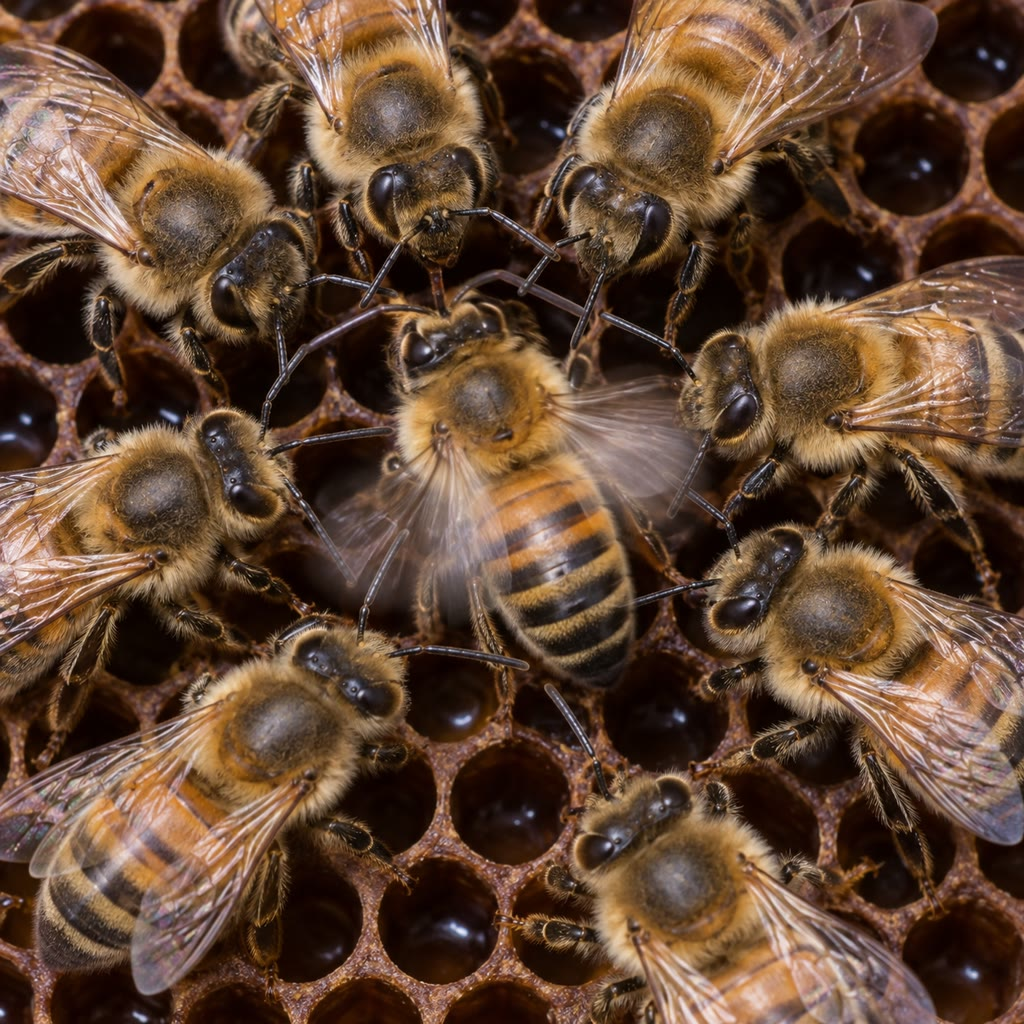
\includegraphics[width=0.4\linewidth]{images/book5/ai/b5-26-bee-dance.jpg}

{\small छत्ते पर नाचती कोई आहार-खोजी, जिसके चारों ओर श्रमिक घेरा बनाए
उसकी दौड़ का कोण तथा ताल पढ़ रहे हैं।}
\end{omfigure}

\begin{remark}[प्राणी गणित करते क्यों लगते हैं]\label{rem:b3:behavioural-ecology:remark}
वह महा टिटहरी $g(t)/(\tau + t)$ का अवकलन नहीं करती, वह मीरकैट $r$ गणित
नहीं करता, और उस मोरनी ने कभी किसी बाधा का नाम नहीं सुना। हर एक ऐसे
नियम ढोता है --- पकड़ धीमी पड़ने पर छोड़ दो, समूह के परिवार होने पर
पुकारो, सबसे चमकीले को पसंद करो --- जिन्हें वरण ने इसलिए गढ़ा कि उनके
पीछे चलते प्राणियों ने अधिक वंशज छोड़े; और वह गणित हमारा है, यानी यह
पूछने का कोई ढंग कि ऐसा होने के लिए उन नियमों को क्या हासिल करना चाहिए,
और उन स्थितियों में व्यवहार का पूर्वानुमान करने का जो उन प्राणियों को
कभी मिली ही नहीं। जब वे पूर्वानुमान विफल हों --- वह टिटहरी बहुत देर रुक
जाए, उस प्रहरी की लागत मानी गई से छोटी निकले --- तब वह विफलता
सूचनाप्रद है: कोई मुद्रा ग़लत थी, कोई बंधन छूट गया, कोई संबंधी ग़लत गिना
गया। यह विषय किसी क्षेत्र-नोटबुक और बीजगणित की किसी पंक्ति के बीच
दशक-दर-दशक चलती कोई बातचीत है, और टिनबर्गन के रखे वे चार प्रश्न दोनों के
लिए वही चौखटा बने हुए हैं।
\end{remark}

\section{अभ्यास}

\begin{exercise}[$\star$]\label{exo:b3:behavioural-ecology:1}
टिनबर्गन के चारों प्रश्न बताइए और लहर-नृत्य के लिए हर एक का एक-एक वाक्य
में उत्तर दीजिए।
\end{exercise}

\begin{exercise}[$\star$]\label{exo:b3:behavioural-ecology:2}
\omterm{def:b3:behavioural-ecology:tinbergen}{नियत क्रिया-प्ररूप} और \omterm{def:b3:behavioural-ecology:tinbergen}{संकेत उद्दीपक} क्या हैं? दो उदाहरण दीजिए और
समझाइए कि तीन लाल पट्टियों वाली उस ``अतिसामान्य'' छड़ी ने क्या दिखाया।
\end{exercise}

\begin{exercise}[$\star$]\label{exo:b3:behavioural-ecology:3}
शब्दों में, \omterm{thm:b3:behavioural-ecology:mvt}{सीमांत मूल्य प्रमेय} क्या कहता है, और यात्रा-काल दुगुना होने
पर वह क्षेत्रक-उपयोग के बारे में क्या पूर्वानुमान करता है?
\end{exercise}

\begin{exercise}[$\star$]\label{exo:b3:behavioural-ecology:4}
ESS परिभाषित कीजिए। शुद्ध कबूतरों की कोई समष्टि ESS क्यों नहीं है, और
बाज़--कबूतर मिश्रण सबको महँगा क्यों पड़ता है?
\end{exercise}

\begin{exercise}[$\star\star$]\label{exo:b3:behavioural-ecology:5}
$V = 6$, $C = 10$ के साथ बाज़--कबूतर: $p^{*}$, उस ESS पर हर रणनीति का
प्रतिफल, और वह प्रतिफल जो सारे कबूतरों की कोई समष्टि पाती, निकालिए।
$V = 12$, $C = 10$ के लिए दोहराइए।
\end{exercise}

\begin{exercise}[$\star\star$]\label{exo:b3:behavioural-ecology:6}
कोई लाभ-फलन $g(t) = A(1 - \mathrm{e}^{-t/T_{0}})$, जिसमें $T_{0} =
\qty{2}{min}$ हो। $t^{*}$ खोजिए, $\tau = 2$ और $\tau = 8$ मिनट के लिए
(अध्याय के मान काम में लीजिए), हर क्षेत्रक का खाया गया अंश, और
दीर्घकालिक दर $R$ प्रति मिनट $A$ के किसी अंश के रूप में।
\end{exercise}

\begin{exercise}[$\star\star$]\label{exo:b3:behavioural-ecology:7}
इनके बीच $r$ निकालिए: सौतेले भाई-बहन; दादा-दादी और पोता-पोती; पहले
चचेरे; कोई अगुणित-द्विगुणित श्रमिक और उसका भाई; और कोई
अगुणित-द्विगुणित रानी तथा उसका बेटा। अंतिम दो समझाइए।
\end{exercise}

\begin{exercise}[$\star\star$]\label{exo:b3:behavioural-ecology:8}
किसी चेतावनी-पुकार से उस पुकारने वाले को मरने की \qty{2}{\%} संभावना
पड़ती है और पास के $n$ संबंधियों में से हर एक \qty{1}{\%} संभावना से बच
जाता है। यदि वे संबंधी सगे भाई-बहन हों तो किस $n$ के लिए \omterm{thm:b3:behavioural-ecology:hamilton}{हैमिल्टन का
नियम} पुकारने का पक्ष लेता है? भतीजियाँ? असंबंधित?
\end{exercise}

\begin{exercise}[$\star\star$]\label{exo:b3:behavioural-ecology:9}
किसी विडोबर्ड की पूँछ \qty{50}{cm} की है; \qty{75}{cm} तक लंबी करने पर
वह दुगुने घोंसले खींचती है, और \qty{25}{cm} तक छोटी करने पर आधे। यदि हर
\qty{25}{cm} जोड़ने पर उत्तरजीविता \qty{20}{\%} गिरे, तो कौन-सी पूँछ
संगमों तथा उत्तरजीविता का गुणनफल अधिकतम करती है, और वह प्राकृतिक पूँछ
उससे छोटी क्यों हो सकती है?
\end{exercise}

\begin{exercise}[$\star\star\star$]\label{exo:b3:behavioural-ecology:10}
कोई तीसरी रणनीति जोड़िए, प्रतिकारी, जो कबूतर की तरह प्रदर्शन करती है पर
हमला होने पर पलटकर लड़ती है। बाज़, कबूतर तथा अपने ही सामने उसके प्रतिफल
लिखिए (बाज़ के सामने वह लड़ती है: $(V - C)/2$; और कबूतर तथा प्रतिकारी
के सामने वह बाँट लेती है: $V/2$)। दिखाइए कि $V < C$ होने पर प्रतिकारियों
की किसी समष्टि पर बाज़ हमला नहीं कर सकते, और चर्चा कीजिए कि क्या कबूतर
उसमें बह सकते हैं।
\end{exercise}

\begin{exercise}[$\star\star\star$]\label{exo:b3:behavioural-ecology:11}
किसी क्षय-युद्ध में हर मुक़ाबलेबाज़ किसी वितरण से खींचे गए समय तक डटा
रहता है; और ESS मध्यमान $V/$(प्रति एकांक समय लागत) वाला चरघातांकी है।
समझाइए कि कोई नियत डटने का समय ESS क्यों नहीं हो सकता, और कोई
चरघातांकी वितरण अब भी प्रदर्शन करते किसी प्रतिद्वंद्वी के प्रत्याशित
आगे के डटने को इससे स्वतंत्र क्यों बना देता है कि वह पहले ही कितनी देर
प्रदर्शन कर चुका है।
\end{exercise}

\begin{exercise}[$\star\star\star$]\label{exo:b3:behavioural-ecology:12}
अगुणित-द्विगुणिता के लिए हैमिल्टन का तर्क पूर्वानुमान करता है कि
श्रमिकों को बहनें ($r = 3/4$) पालना पसंद होना चाहिए, न कि भाई
($r = 1/4$), जबकि वह रानी बेटों तथा बेटियों को बराबर मूल्य देती है। यदि
वह नियंत्रण श्रमिकों के हाथ हो और यदि रानी के, तो किसी बस्ती को जो
प्रजननक्षम पैदा करने चाहिए उनका लिंग-अनुपात पूर्वानुमानित कीजिए; बताइए
कि ट्राइवर्स तथा हेयर ने क्या पाया, और कोई ऐसी रानी, जो कई नरों से संगम
करे, उस तर्क का क्या करती है।
\end{exercise}

\section{समस्या: प्रहरी का अंकगणित}

\begin{problem}[{सप्तांत समस्या --- किसी मीरकैट समूह का एक दिन
व्यवहार-पारिस्थितिकी की तरह किया गया: सीमांत मूल्य प्रमेय के
क्षेत्रक-काल, बाज़--कबूतर क्रीड़ा तथा उसके ESS के मुक़ाबले,
प्रहरी-ड्यूटी का और किसी अगुणित-द्विगुणित छत्ते का बंधु-लेखा, और किसी
आभूषण की लागत, जिसका अंत क्षेत्रक-निवास काल पर होता है, बाज़-बारंबारता
पर, और प्रहरी की हैमिल्टन-देहली पर}]
\label{pb:b3:behavioural-ecology:1}
आँकड़े: आहार-खोज के क्षेत्रक, जिनका $g(t) = A(1 - \mathrm{e}^{-t/T_{0}})$, $T_{0}
= \qty{3}{min}$, $A = \qty{60}{kJ}$; क्षेत्रकों के बीच यात्रा $\tau =
\qty{3}{min}$ (सघन आवास) या \qty{12}{min} (विरल)। किसी बिल पर
मुक़ाबले: $V = 10$, $C = 30$ (सुयोग्यता मात्रक)। प्रहरी: घंटे भर की ड्यूटी
उस प्रहरी को $c = 0.03$ संतति-तुल्य (खोया भोजन, संसर्ग) की पड़ती है; वह
हर समूह-साथी का परभक्षण-जोखिम घटाती है, जिसका मूल्य हर एक के लिए
$b = 0.01$ संतति-तुल्य है; और उस समूह के $n$ सदस्य हैं जिनकी औसत
संबंधिता $\bar r$ है। छत्ता: कोई श्रमिक उसी प्रयास से या तो $k$ बहनें
पाल सकती है या $k$ अपनी बेटियाँ। आभूषण: पूँछ की लंबाई $L$ संगम
$m(L) = L/20$ और उत्तरजीविता $s(L) = 1 - (L/100)^{2}$ देती है, और $L$
cm में।

\medskip
\noindent\textbf{भाग I --- क्षेत्रक।}
\begin{enumerate}
  \item दीर्घकालिक दर $R(t)$ और इस $g$ के लिए सीमांत मूल्य की शर्त
        लिखिए।
  \item दिखाइए कि वह शर्त $(\tau + t)/T_{0} = \mathrm{e}^{t/T_{0}}
        - 1$ बन जाती है, और उसे $\tau = T_{0}$ के लिए हल कीजिए
        ($t = 1.15\,T_{0}$ आज़माइए)।
  \item $\tau = 4T_{0}$ के लिए हल कीजिए ($t = 2.0\,T_{0}$ आज़माइए)।
  \item हर स्थिति के लिए: मिनटों में निवास-काल, प्रति क्षेत्रक ऊर्जा,
        उस क्षेत्रक का खाया गया अंश, और दर $R$ kJ/min में।
  \item कोई अंगूठा-नियम: ``नियत \qty{5}{min} के बाद छोड़ दो।'' दोनों
        आवासों के लिए $R$ निकालिए और उस इष्टतम से तुलना कीजिए। क्या वह
        नियम काफ़ी अच्छा है?
  \item कोई दूसरा नियम: ``जब \qty{20}{s} बिना किसी पकड़ के बीत जाएँ तब
        छोड़ दो।'' समझाइए कि यह छोड़ने-के-समय वाला नियम उस प्रमेय के
        पास क्यों आता है, और क्षेत्रकों की समृद्धि भिन्न होने पर वह किस
        दिशा में विफल होता है।
\end{enumerate}

\medskip
\noindent\textbf{भाग II --- मुक़ाबले।}
\begin{enumerate}[resume]
  \item प्रतिफल-आव्यूह लिखिए और $p^{*}$ निकालिए।
  \item $p = 0.1$, $p = p^{*}$ और $p =
        0.6$ पर बाज़ तथा कबूतर का प्रतिफल; हर स्थिति में कौन-सी रणनीति
        फैलती है?
  \item उस ESS पर प्रतिफल; सारे-कबूतर प्रतिफल से तुलना कीजिए। लड़ने की
        संभावना के कारण वह समष्टि प्रति मुक़ाबला कितना खोती है?
  \item किसी सूखे से $V$ चढ़कर $40$ हो जाता है (बिल दुर्लभ)। नया ESS?
        यह कठिन वर्षों की लड़ाइयों के बारे में क्या पूर्वानुमान करता है?
  \item बुर्जुआ: ``निवासी हो तो बाज़, घुसपैठिया हो तो कबूतर,'' और हर
        भूमिका आधा-आधा समय। अपने ही सामने उसका प्रतिफल बिना किसी लड़ाई
        के $V/2$ है। दिखाइए कि $V
        < C$ होने पर बाज़ किसी बुर्जुआ समष्टि पर हमला नहीं कर सकते, और
        उस चित्तीदार वन-तितली की व्याख्या कीजिए।
  \item एक वाक्य में समझाइए कि इस व्यवहार पर किसी इष्टतम का नहीं बल्कि
        बारंबारता-निर्भरता का शासन क्यों है।
\end{enumerate}

\medskip
\noindent\textbf{भाग III --- बंधु।}
\begin{enumerate}[resume]
  \item उस प्रहरी के लिए \omterm{thm:b3:behavioural-ecology:hamilton}{हैमिल्टन का नियम}: $n\bar r$ पर शर्त। किस
        $n\bar r$ के लिए वह ड्यूटी फ़ायदेमंद है?
  \item $n = 8$ सगे भाई-बहनों का कोई समूह ($\bar r = 1/2$): क्या वह
        फ़ायदेमंद है? 8 असंबंधित प्राणियों का कोई समूह? 8 सौतेले
        भाई-बहनों का कोई समूह?
  \item वह प्रहरी अच्छी तरह खाया हुआ है, इसलिए उसका $c$ गिरकर
        $0.01$ रह जाता है। अब देहली? यह पूर्वानुमान क्यों करता है कि
        प्रहरी वे व्यष्टि होते हैं जो अच्छी तरह खाए हुए हैं?
  \item वह छत्ता: $k$ बहनों का $k$ बेटियों के सामने समावेशी-सुयोग्यता
        मूल्य। किसी श्रमिक को कौन-सी पसंद करनी चाहिए, और किस अनुपात से?
  \item उस रानी ने तीन नरों से बराबर संगम किया है: बहनों से श्रमिकों की
        औसत संबंधिता? क्या वह पसंद बची रहती है?
  \item समझाइए कि हैमिल्टन के नियम को उस कर्ता से बंधुओं की पहचान की
        माँग क्यों नहीं है, और कोई भू-गिलहरी असल में कौन-सा अंगूठा-नियम
        काम में ले सकती है।
\end{enumerate}

\medskip
\noindent\textbf{भाग IV --- आभूषण।}
\begin{enumerate}[resume]
  \item सुयोग्यता $W(L) = m(L)\,s(L)$। $W$ निकालिए, $L = 20$, $40$, $60$,
        $80$ के लिए।
  \item वह $L$ खोजिए जो $W$ को विश्लेषणात्मक रूप से अधिकतम करे, और वहाँ
        $W$।
  \item उत्तरजीविता-लागत तीखी होकर $s = 1 - (L/70)^{2}$ हो जाती है (कोई
        परभक्षी आ जाता है)। नया इष्टतम? किस दिशा में, और यह उस पूँछ के
        विकास के परभक्षण के पीछे चलने का पूर्वानुमान क्यों करता है?
  \item ऐंडरसन के प्रयोग ने पूँछें दुगुनी करके \qty{75}{cm} कीं और
        घोंसले दुगुने किए। लंबी पूँछों के लिए मादा की वह पसंद, जो
        ``इष्टतम से आगे'' है, भगोड़े हिसाब से संगत है, बाधा-हिसाब से, या
        दोनों से?
  \item कोई सस्ता आभूषण कोई \omterm{prop:b3:behavioural-ecology:signals}{ईमानदार संकेत} क्यों नहीं है, और प्रश्न~21
        की वह लागत उसे ईमानदार कैसे बना देती है?
  \item \omterm{def:b3:behavioural-ecology:sexual-selection}{बेटमैन प्रवणताएँ}: नर हर अतिरिक्त संगम पर $0.8$ संतति पाते हैं,
        मादाएँ $0.1$। किसी एक अनुच्छेद में समझाइए कि यह असममिति भाग~II
        के मुक़ाबले और भाग~IV के आभूषण, दोनों कैसे पैदा करती है।
  \item सारांश दीजिए: सघन आवास में $t^{*}$ (प्रश्न~4), $p^{*}$
        (प्रश्न~7), और प्रहरी की देहली $n\bar r$
        (प्रश्न~13)।
\end{enumerate}
\end{problem}
